\documentclass[10pt]{article}

\usepackage{spheric}
%%%TITLE
\title{Stable sharp interface method for SPH}
\date{}

%%AFFILIATIONS
\author[$\relax$]{Stable sharp interface method for SPH}

\affil[$\relax$]{Institute of Applied Physics and Computational Mathematics, Beijing, China}

\affil[$\relax$]{\href{mailto:zhang_mingyu@iapcm.ac.cn}{zhang\_mingyu@iapcm.ac.cn}}


%%DOCUMENT
\begin{document}

\maketitle

%\SelectedTopics{}

%%PLEASE PUT YOUR ABSTRACT HERE
\begin{abstract}
Interface is a key issue in the study of multiphase flows existing in our daily life and industrial applications. Many mesh methods have been developed to treat the interface, including Level set method (LSM), volume of fluid (VOF), front tracking method (FT), and phase field method, et al. As a meshfree method, Smoothed Particle Hydrodynamics (SPH) can easily handle complex flows with interface.

In Zhang and Deng's previous work \cite{zhang2015sharp}, a sharp interface method (SIM) based on level set method and ghost fluid method is presented for SPH. The level set method is used to describe the interface. Based on level set method, the calculation of the interface normal vector and curvature has higher performance. And the ghost fluid method is introduced to handle the discontinuity. The interface states are obtained by using of the jump conditions at the interface and are extended to the ghost fluid particles. The ghost fluid method improves the stability and smoothness of calculation around the interface.

Based on the Lagrangian nature of SPH, a new method for locating the interface is presented. Because the Lagrangian nature of SPH guarantees mass conservation of each phase around the interface, the new interface method for SPH is more efficient and stable.

In this talk, the new developed interface method for SPH is presented. The numerical behavior of the new method is shown by benchmark tests. The new method and its future version can be used to study the complex flows.

\begin{figure}[!htb]
\centering
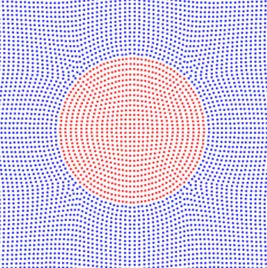
\includegraphics[width=0.45\textwidth]{21-1.png}
\caption{Square drop at stable state.}\label{fig:21}
\end{figure}

\end{abstract}


%%THE END OF ABSTRACT

\addbib

\end{document}
